%\normalsize
In the era of the Higgs discovery and scrupulous searches
for signals of new physics at the LHC it is crucial
to have accurate Standard Model (SM) predictions for
many hard scattering processes such as the Higgs production at the LHC.
A most common approach to calculate the SM cross sections for  
such reactions is to use perturbative QCD collinear factorisation:
%is with perturbative QCD using a (collinear) factorisation approach: 
%{\small
\begin{equation}
\small
\begin{array}{lcl}
\sigma^{pp\rightarrow H + X}(\alpha_s,\mu_r,\mu_f) & = &
\sum\limits_{a,b}\,  \int\limits_{0}\limits^{1} dx_1 \int\limits_{0}\limits^{1} dx_2\, f_a(x_1,\alpha_s,\mu_F) 
 f_b(x_2,\alpha_s,\mu_F)\\ 
& \times & \, \hat{\sigma}^{ab \rightarrow H + X}(x_1,x_2;\alpha_s,\mu_R,\mu_F).
%\sigma^{pp\rightarrow H + X}(\alpha_s,\mu_r,\mu_f) = 
%\sum_{a,b} \int_{0}^{1} dx_1 \int_{0}^{1} dx_2 f_a(x_1) 
% f_b(x_1,\alpha_s,\mu_F) \times \hat{\sigma}^{ab \rightarrow H + X}(x_1,x_2;\alpha_s,\mu_R,\mu_F)
\label{eq:fact}
\end{array}
\end{equation}
%}
Here the cross section $\sigma^{pp\rightarrow H + X}$ for inclusive
Higgs production is expressed
as a convolution of Parton Distribution Functions (PDF) $f_a$ and $f_b$
with the partonic cross section
% that describe
%the 
$\hat{\sigma}^{ab \rightarrow H + X}$.
%
The PDFs describe 
the probability of finding a specific parton $a$ ($b$) in the first (second) proton carrying the fraction $x_1$ ($x_2$) of its momentum.
%
The sum in Eq.~\ref{eq:fact} in indeces $a$ and $b$ is over all different kind of partons,
i.e. gluons and the various quarks and antiquarks flavours, that are considered
as the constituents of the proton.
%
Both the PDFs and the partonic cross section depend on the strong coupling
constant $\alpha_s$, the factorisation and renormalisation scales,
$\mu_F$ and $\mu_R$, respectively.
%
The partonic cross sections are calculable in pQCD while
the PDFs cannot be determined solely with pQCD but are assumed 
to be universal.
%
This permits the use of different scattering reactions 
to constrain the PDFs; in particular one can use specific reaction data 
for determining the PDFs and then take these PDFs for
predicting other processes via Eq.~\ref{eq:fact}.
%

Key information on the PDFs is provided by the Deep Inelastic Scattering (DIS) data from the $ep$ collider HERA.
%
For instance, the gluon density relevant
for calculating the dominant gluon-gluon fusion contribution to the Higgs production
at the LHC can be accurately determined from the HERA data alone.
%
%Despite being often plagued by larger perturbative uncertainties,
Specific data from the Tevatron $p\bar{p}$ and the LHC $pp$ collider
can help to further constrain the PDFs.
%
The most sensitive processes at the  $p\bar{p}$ colliders are
Drell Yan production, W and Z asymmetries, top quark production, and jet production.
%

\fitter represents a QCD analysis framework that aims at 
determining precise PDFs by integrating all the PDF sensitive information
from HERA, Tevatron and the LHC.
%
The processes that are currently included in \fitter framework are listed in Tab.~\ref{tab:proc}.
%
\begin{table}
\small
%\tiny
\scriptsize

\begin{tabular}{|l|l|l|l|}
\hline
Data &Type &  Reaction & Theory      \\
        &     &     & calculation \\
\hline

HERA &DIS NC   &$ep\to ep$ & QCDNUM, RT, ACOT \\
HERA &DIS CC   &$ep\to \nu_e p$ & QCDNUM, RT, ACOT\\
HERA &DIS jets &$ep\to eX$ & FastNLO (NLOJet++)\\
HERA &DIS heavy quark & $ep\to ep $& ZM (QCDNUM), RT, ACOT, \\
     &                     &            & FFNS (ABM,QCDNUM) \\
\hline
Fixed Target &DIS NC   &$ep\to ep$ & ZM (QCDNUM), RT, ACOT \\
\hline
Tevatron, LHC &Drell Yan &$pp(\bar p)$ & APPLGRID (MCFM) \\
Tevatron, LHC &W charge asym &$pp(\bar p)$ & APPLGRID (MCFM) \\
Tevatron, LHC &top &$pp(\bar p)$ & APPLGRID (MCFM),  \\
              &    &             & HATHOR \\
Tevatron, LHC &jets &$pp(\bar p)$ & APPLGRID (NLOJet++) \\
                &  & & FastNLO (NLOJet++) \\
LHC&  DY+heavy quark &$pp(\bar p)$ & APPLGRID (MCFM) \\
\hline
\end{tabular}
\caption{The list of processes available in \fitter.}
\label{tab:proc}
\end{table}
%
\normalsize
The basic functionality of HERAFitter is shown in Fig.~\ref{fig:flow} and consists of four parts: %{\bf needs to update figure!}
\begin{figure}[!ht]
   \centering
   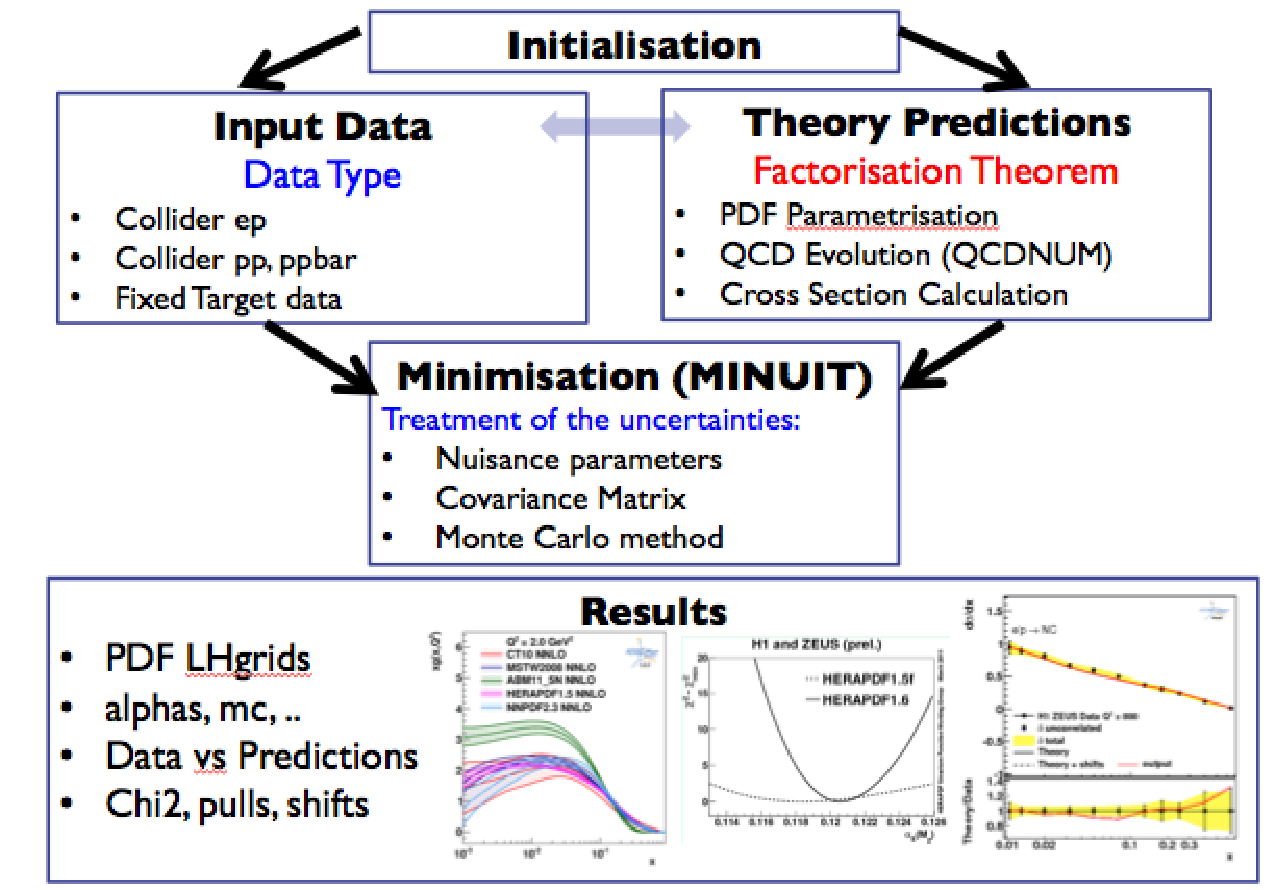
\includegraphics[width=8cm]{flow.pdf}
   \caption{Schematic structure of the \fitter program.} 
 \label{fig:flow}
\end{figure}
\begin{description}
\item 
\bf {Input data:} \rm  All relevant cross section data from the various reactions
are stored internally in \fitter with the full information on their uncorrelated and correlated
uncertainties.
\item
\bf{Theory predictions:} \rm Predictions are obtained relying on factorisation approach (Eq.~\ref{eq:fact}). PDFs are parametrised at a starting scale $Q_0$  by a chosen functional form with a set of free parameters $\vec{p}$. Then they evolved from $Q_0$ to the scale of the measurement using 
Dokshitzer-Gribov-Lipatov-Altarelli-Parisi 
(DGLAP)~\cite{Gribov:1972ri, Gribov:1972rt, Lipatov:1974qm,
Dokshitzer:1977sg, Altarelli:1977zs} evolution equations 
as implemented in QCDNUM~\cite{qcdnum}, 
and then multiplied (Eq.~\ref{eq:fact}) with the hard parton cross sections calculated by
a specific theory program (also listed in Tab.~\ref{tab:proc}).
\item
\bf{Minimization:} \rm  PDFs are extracted from a least square fit by constructing a 
$\chi^2$ from the input data and the theory prediction.
The $\chi^2$ is  minimized iteratively 
with respect to the PDF parameters using the MINUIT\cite{minuit} program.
%
%Fitted values of $\vec{p}$ and estimated uncertainties are obtained.
%The fitted parameters $\vec(p)$ and obtained from the uncertainties of the parameters are determined (from chi2+1???)
%
\item
\bf{Results:} \rm  The fitted parameters $\vec{p}$ and their estimated uncertainties are produced.
The resulting PDFs are provided in a ready to be used LHAPDF library format
and can be graphically 
displayed at arbitrary scales with their one sigma uncertainties bands.
To demonstrate the fit consistency, plots are provided 
in which the input data are compared to the fitted theory predictions. This is also illustrated in the figure ~\ref{fig:data} using for demonstration HERA I data (the default sets in \fitter) compared to predictions based on HERAPDF1.0\cite{h1zeus:2009wt}.  
\begin{figure}[!ht]
   \centering
   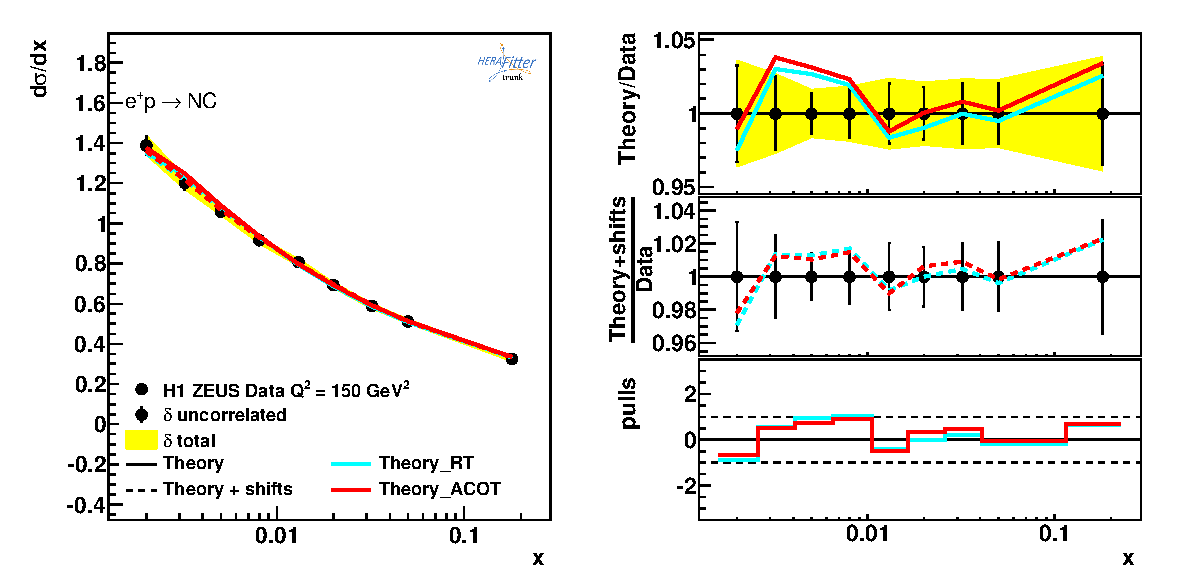
\includegraphics[width=8cm]{datatheory.pdf}
   \caption{An illustration of results output using drawing tools from \fitter which compares the measurements (in this case HERA I) to the predictions or fit. In addition, ratio plots are also provided together with the pull distribution (left panel).} 
 \label{fig:data}
\end{figure}

\end{description}
%
%This paper provides a comprehensive description of  \\
%the \fitter\ package.
%which is designed for analysis of the High Energy Physics data.
%The package has been developed by members of the H1 and ZEUS collaborations
%with an exclusive support of different theoretical groups.
%The main purpose of the \fitter\ package is analysis of the 
%data from the $e^{\pm}p$, $p\bar{p}$, and $pp$ collider experiments
%information obtained from the deep inelastic scattering experiments
%and the determination of the parton density functions (PDFs).
%The broad range of data taken from the $e^{\pm}p$, $p\bar{p}$, and $pp$ collider experiments can be
%studied by the package. 

%Based on the concept of factorisable nature of the cross sections into universal parton distribution functions (PDFs) and process dependent partonic scattering cross sections, 

The \fitter\ program permits determination of the PDFs from the variours measurements of the cross section at $ep$, $p\bar{p}$ or $pp$ colliders.  
 It includes various options for theoretical models and choices to account for the experimental uncertainties. Therefore, this project represents not only an ideal environment for benchmarking studies, but also a unique support for the QCD interpretation of analyses within the LHC experiments,
as already demonstrated by several publicly available results using the \fitter\ 
framework~\cite{atlas:strange,atlas:jets,atlas:hm,cms:strange,cms:jets,h1:2012kk,h1zeus:charm}.  

The outline of this paper is as follows.
%
Section~\ref{sec:theory} discusses the various processes 
and corresponding theoretical calculations performed in the Dokshitzer-Gribov-Lipatov-Altarelli-Parisi (DGLAP)~\cite{Gribov:1972ri,Gribov:1972rt,Lipatov:1974qm,
Dokshitzer:1977sg,Altarelli:1977zs} formalism that are available in \fitter.
The alternative approaches to the DGLAP formalism are presented in section~\ref{sec:alternative}.
%
In section~\ref{sec:techniques} various techniques in invoking the theory calculations are described.
Section~\ref{sec:method} elucidates the 
methodology of determining PDFs through fits based on various
% {\bf (what do you mean here
%by approaches?)} 
 $\chi^2$ definitions used in the
minimisation procedure. 
%
Specific applications of the package are given in
section ~\ref{sec:examples}. 
%
%{\bf add something more here?.}
